
%%%%%%%%%%%%%%%%%%%%%%% file template.tex %%%%%%%%%%%%%%%%%%%%%%%%%
%
% This is a general template file for the LaTeX package SVJour3
% for Springer journals.          Springer Heidelberg 2010/09/16
%
% Copy it to a new file with a new name and use it as the basis
% for your article. Delete % signs as needed.
%
% This template includes a few options for different layouts and
% content for various journals. Please consult a previous issue of
% your journal as needed.
%
%%%%%%%%%%%%%%%%%%%%%%%%%%%%%%%%%%%%%%%%%%%%%%%%%%%%%%%%%%%%%%%%%%%
%
% First comes an example EPS file -- just ignore it and
% proceed on the \documentclass line
% your LaTeX will extract the file if required
\begin{filecontents*}{example.eps}
%!PS-Adobe-3.0 EPSF-3.0
%%BoundingBox: 19 19 221 221
%%CreationDate: Mon Sep 29 1997
%%Creator: programmed by hand (JK)
%%EndComments
gsave
newpath
  20 20 moveto
  20 220 lineto
  220 220 lineto
  220 20 lineto
closepath
2 setlinewidth
gsave
  .4 setgray fill
grestore
stroke
grestore
\end{filecontents*}
%
\RequirePackage{fix-cm}
%
\documentclass{svjour3}                     % onecolumn (standard format)
%\documentclass[smallcondensed]{svjour3}     % onecolumn (ditto)
%\documentclass[smallextended]{svjour3}       % onecolumn (second format)
%\documentclass[twocolumn]{svjour3}          % twocolumn
%
\smartqed  % flush right qed marks, e.g. at end of proof
%
\usepackage{graphicx}
%
% \usepackage{mathptmx}      % use Times fonts if available on your TeX system
%
% insert here the call for the packages your document requires
%\usepackage{latexsym}
% etc.
%
% please place your own definitions here and don't use \def but
% \newcommand{}{}
%
% Insert the name of "your journal" with
% \journalname{myjournal}
%
\begin{document}

\title{The Pandora multi-algorithm approach to automated pattern recognition of cosmic-ray muon and test beam events in the ProtoDUNE-SP detector
%\thanks{Grants or other notes
%about the article that should go on the front page should be
%placed here. General acknowledgments should be placed at the end of the article.}
}
%\subtitle{Do you have a subtitle?\\ If so, write it here}

%\titlerunning{Short form of title}        % if too long for running head

\author{First Author         \and
        Second Author %etc.
}

%\authorrunning{Short form of author list} % if too long for running head

\institute{F. Author \at
              first address \\
              Tel.: +123-45-678910\\
              Fax: +123-45-678910\\
              \email{fauthor@example.com}           %  \\
%             \emph{Present address:} of F. Author  %  if needed
           \and
           S. Author \at
              second address
}

\date{Received: date / Accepted: date}
% The correct dates will be entered by the editor


\maketitle

\begin{abstract}
Insert your abstract here. Include keywords, PACS and mathematical
subject classification numbers as needed.
\keywords{First keyword \and Second keyword \and More}
% \PACS{PACS code1 \and PACS code2 \and more}
% \subclass{MSC code1 \and MSC code2 \and more}
\end{abstract}

\section{Introduction}
\label{intro}
Your text comes here. Separate text sections with

-Abstract and introduction, covering Pandora background, its use across LArTPC programme, ProtoDUNE and aspects of the pattern recognition problem specific to ProtoDUNE.
-ProtoDUNE details.
-Pattern recognition. We?d reference the MicroBooNE algorithm description, give an executive summary of PandoraCosmic and explain how PandoraTestBeam differs from PandoraNu. In the MicroBooNE paper, we used a two-pass reconstruction, but explicitly said that this would become more sophisticated soon. This then allows us to explain the consolidated reconstruction properly, making this a major communication goal of the paper. Includes stitching, more on slicing, beam particle id.
-Performance assessment, using MC and metrics consistent with MicroBooNE paper to assess quality of pattern recognition, understand contributions to efficiency, etc., but then moving into real data plots. Inclusion of all of the latest and greatest plots, with (ideally!) explanation of the key features.
-Concluding comments (short).

\section{ProtoDUNE-SP}
\label{sec:1}
Text with citations \cite{RefB} and \cite{RefJ}.
\subsection{Subsection title}
\label{sec:2}
as required. Don't forget to give each section
and subsection a unique label (see Sect.~\ref{sec:1}).
\paragraph{Paragraph headings} Use paragraph headings as needed.
\begin{equation}
a^2+b^2=c^2
\end{equation}

\section{Pattern Recognition}

\subsection{Algorithm Chains}

\subsubsection{Pandora Test Beam}

Reference the basis as Pandora Neutrino.  Highlight test beam particle creation algorithm.  Add lots of pictures of both tracks and shower events.

\subsubsection{Pandora Cosmic}

Mention stitching here. 

Reference the MicroBooNE paper.

\subsection{Consolidated Reconstruction}

The consolidated reconstruction is a framework designed to reconstruct test beam particles in the presence of cosmic ray backgrounds.  The process utilises both the Pandora Teat Beam and Cosmic algorithm chains in order to apply the optimal pattern recognition logic to any given scenario.   

The consolidated reconstruction begins by running the Pandora Cosmic algorithm chain that reconstructs all particles under the cosmic ray particle hypothesis.  The reconstructed particles are then examined in order to determine if they are clear cosmic rays.  Two distinct methods are used for identifying clear cosmic rays:

\begin{itemize}
\item If the hits for the reconstructed particle fall outside the expected read out time window for the target test beam particle.
\item If it the reconstructed particle enters the detector through the top face and exists the lower face.  
\end{itemize}


\section{Assessment of Pattern Recognition}

\subsection{Monte-Carlo}

\subsubsection{Test Beam Metrics}

\begin{figure}
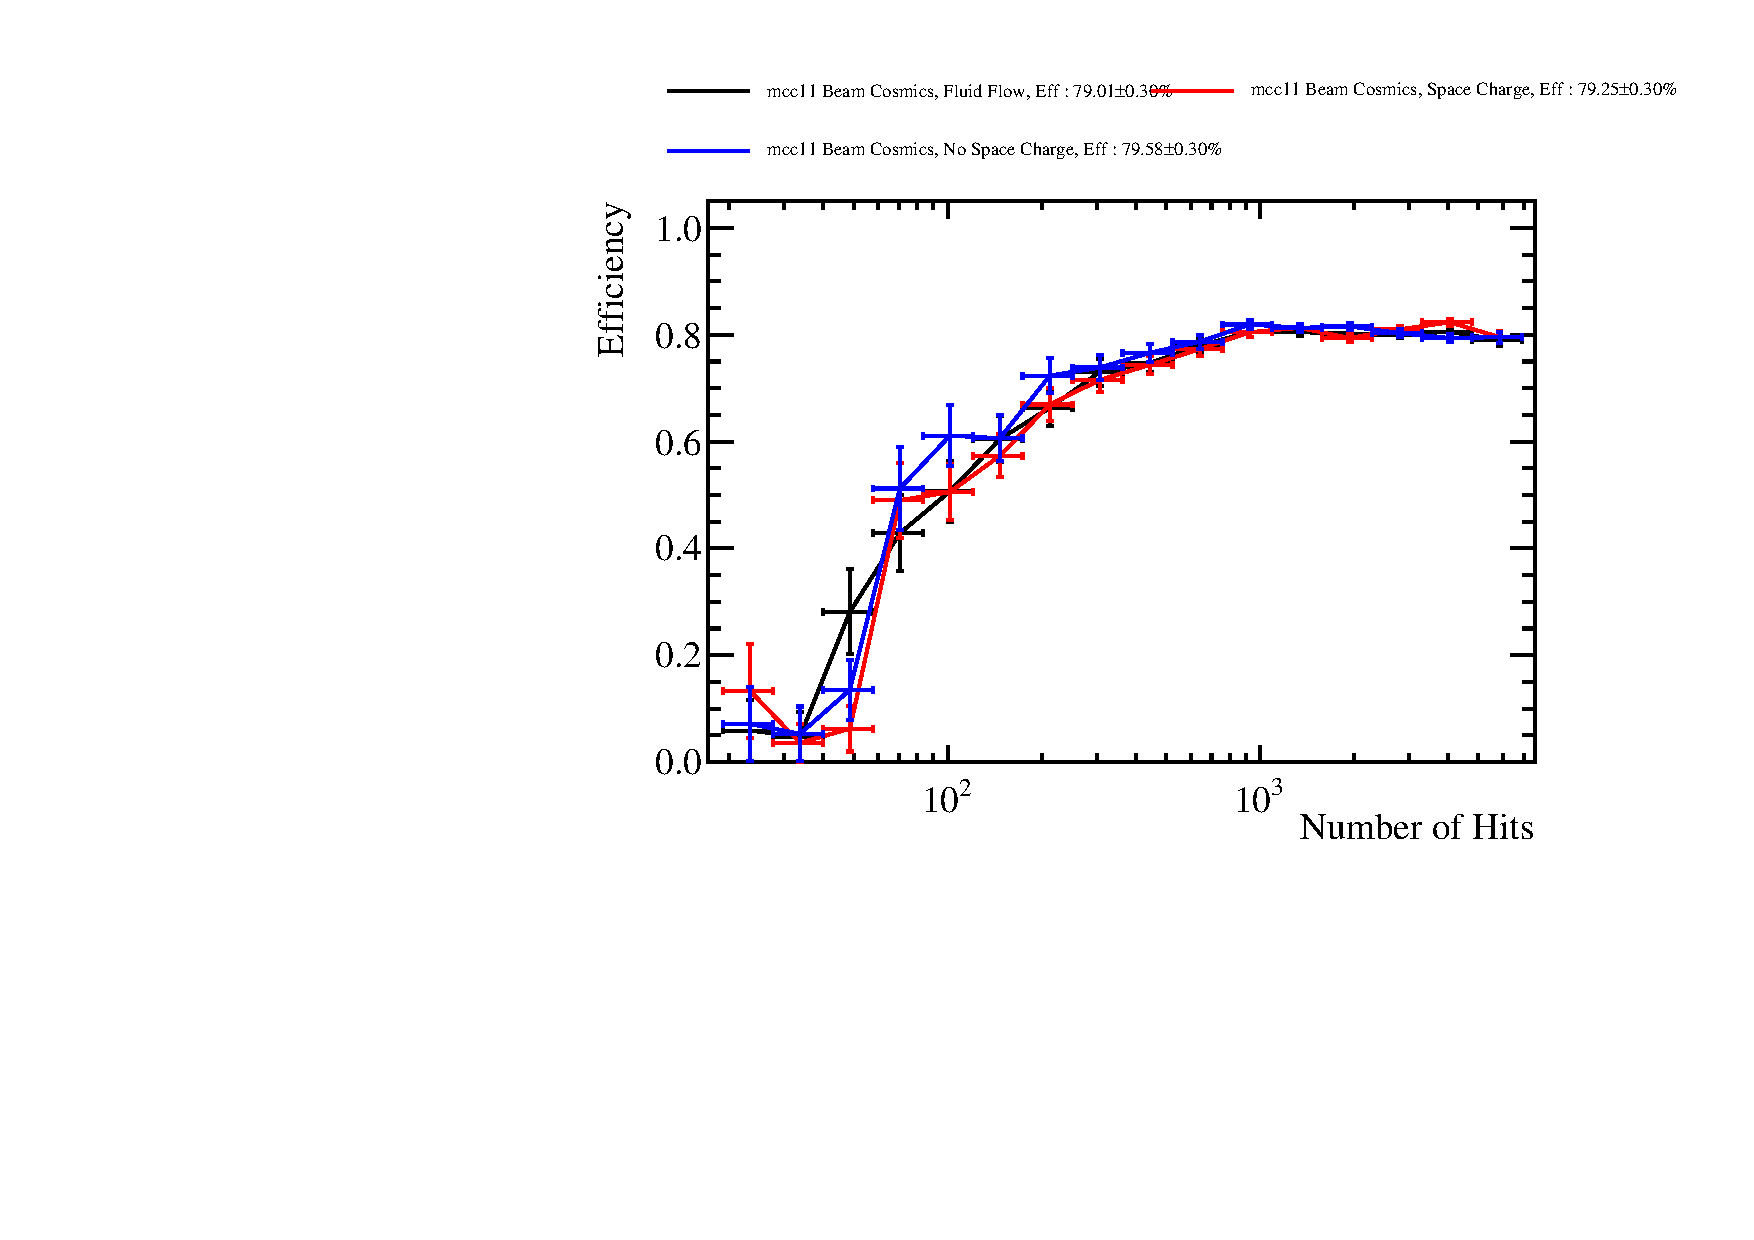
\includegraphics[width=0.5\textwidth]{Figures/Metrics/MC/Beam/BeamParticleEfficiencyBreakdownVsNHits.pdf}
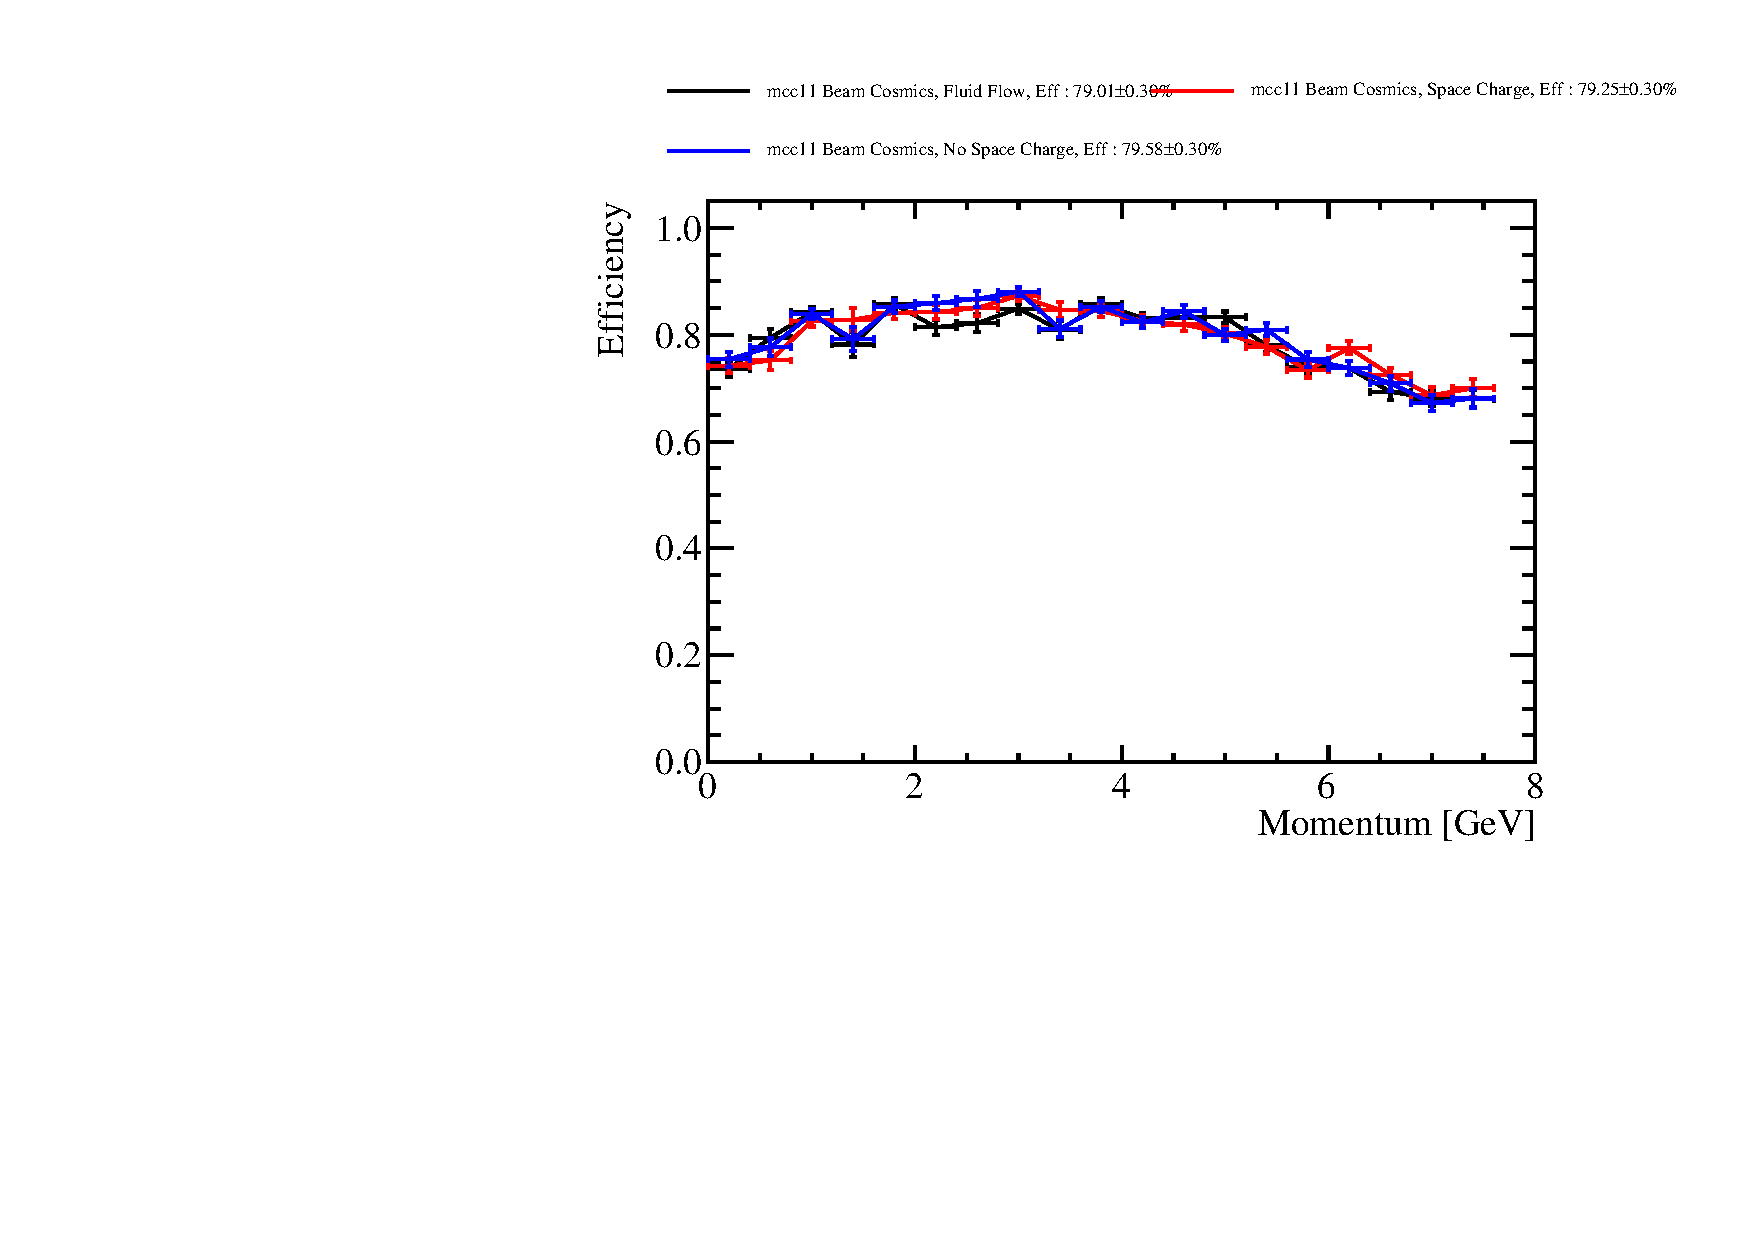
\includegraphics[width=0.5\textwidth]{Figures/Metrics/MC/Beam/BeamParticleEfficiencyBreakdownVsMomentum.pdf}
\caption{Please write your figure caption here}
\label{fig:1}
\end{figure}

\begin{figure}
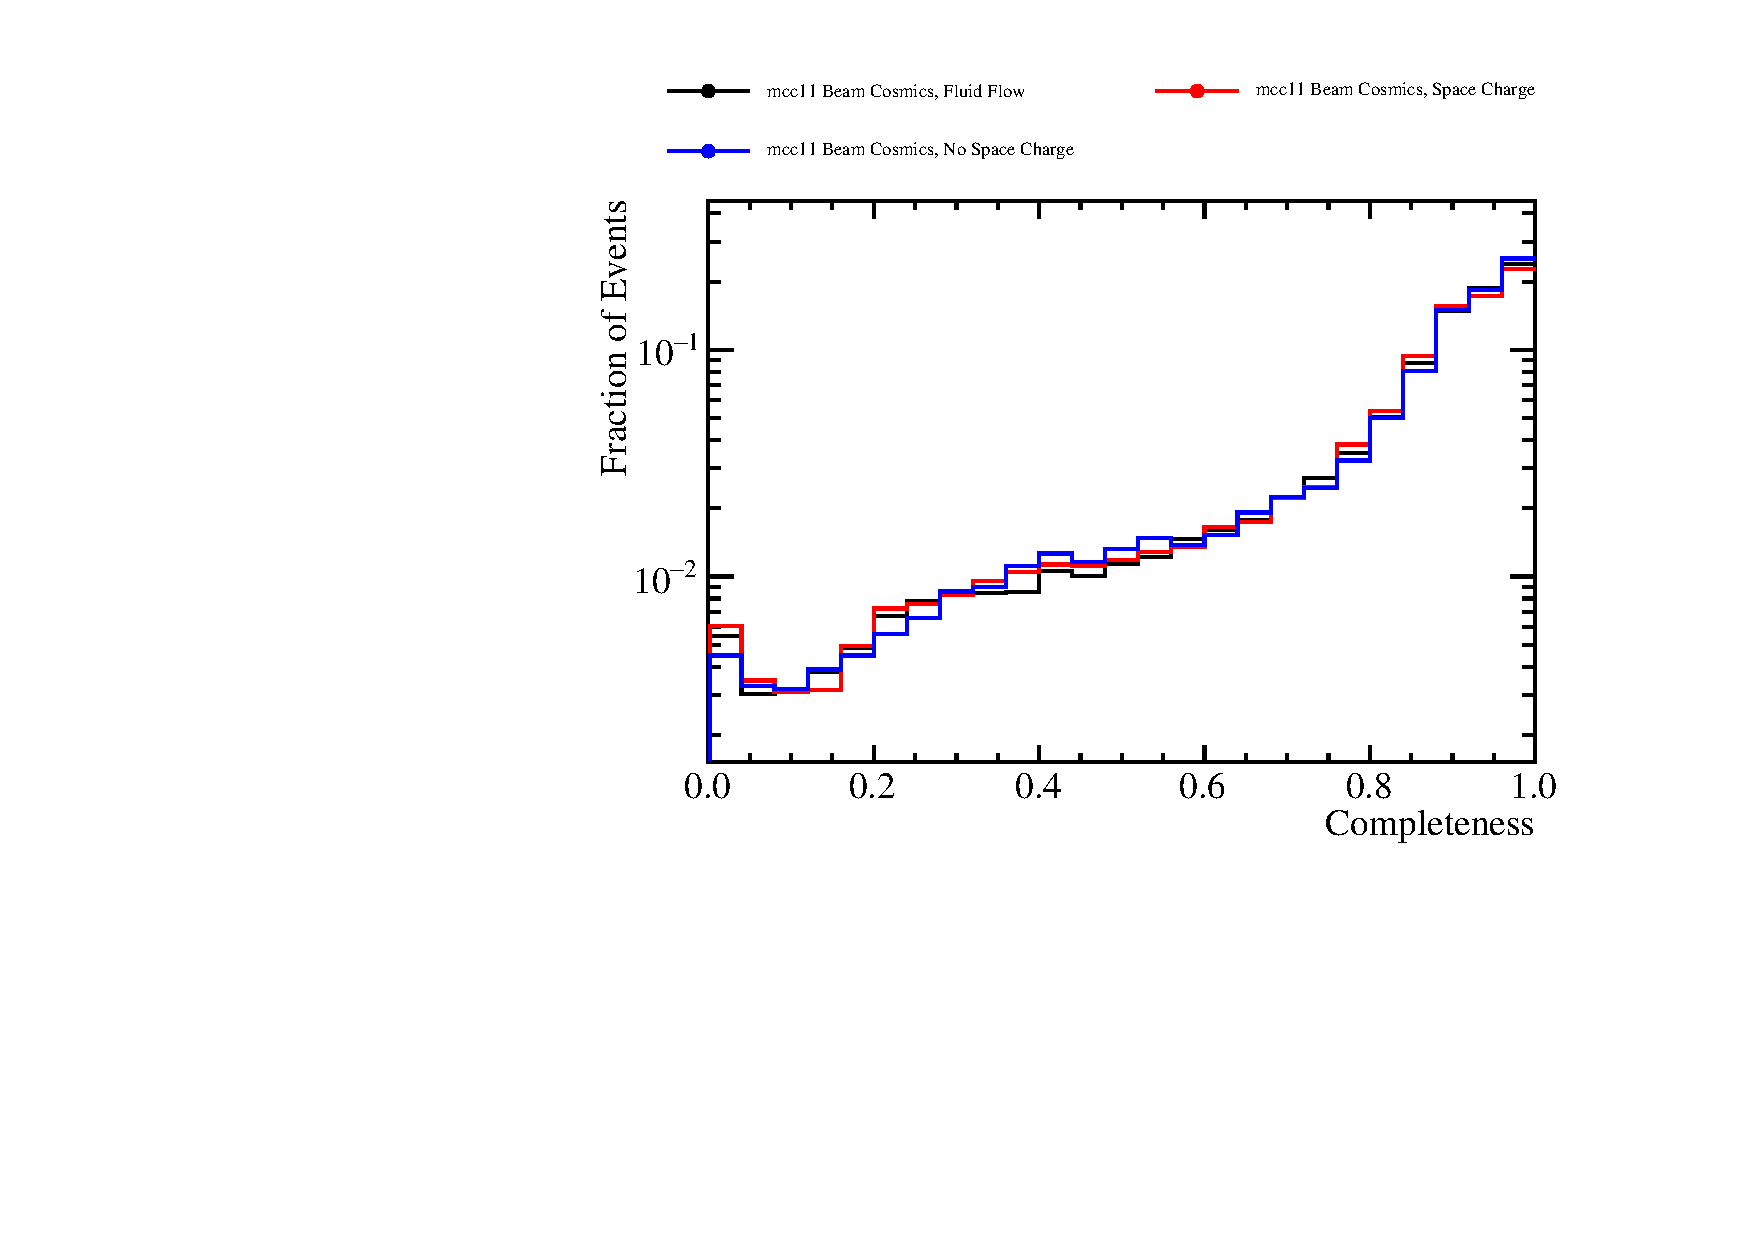
\includegraphics[width=0.5\textwidth]{Figures/Metrics/MC/Beam/BeamParticleCompleteness.pdf}
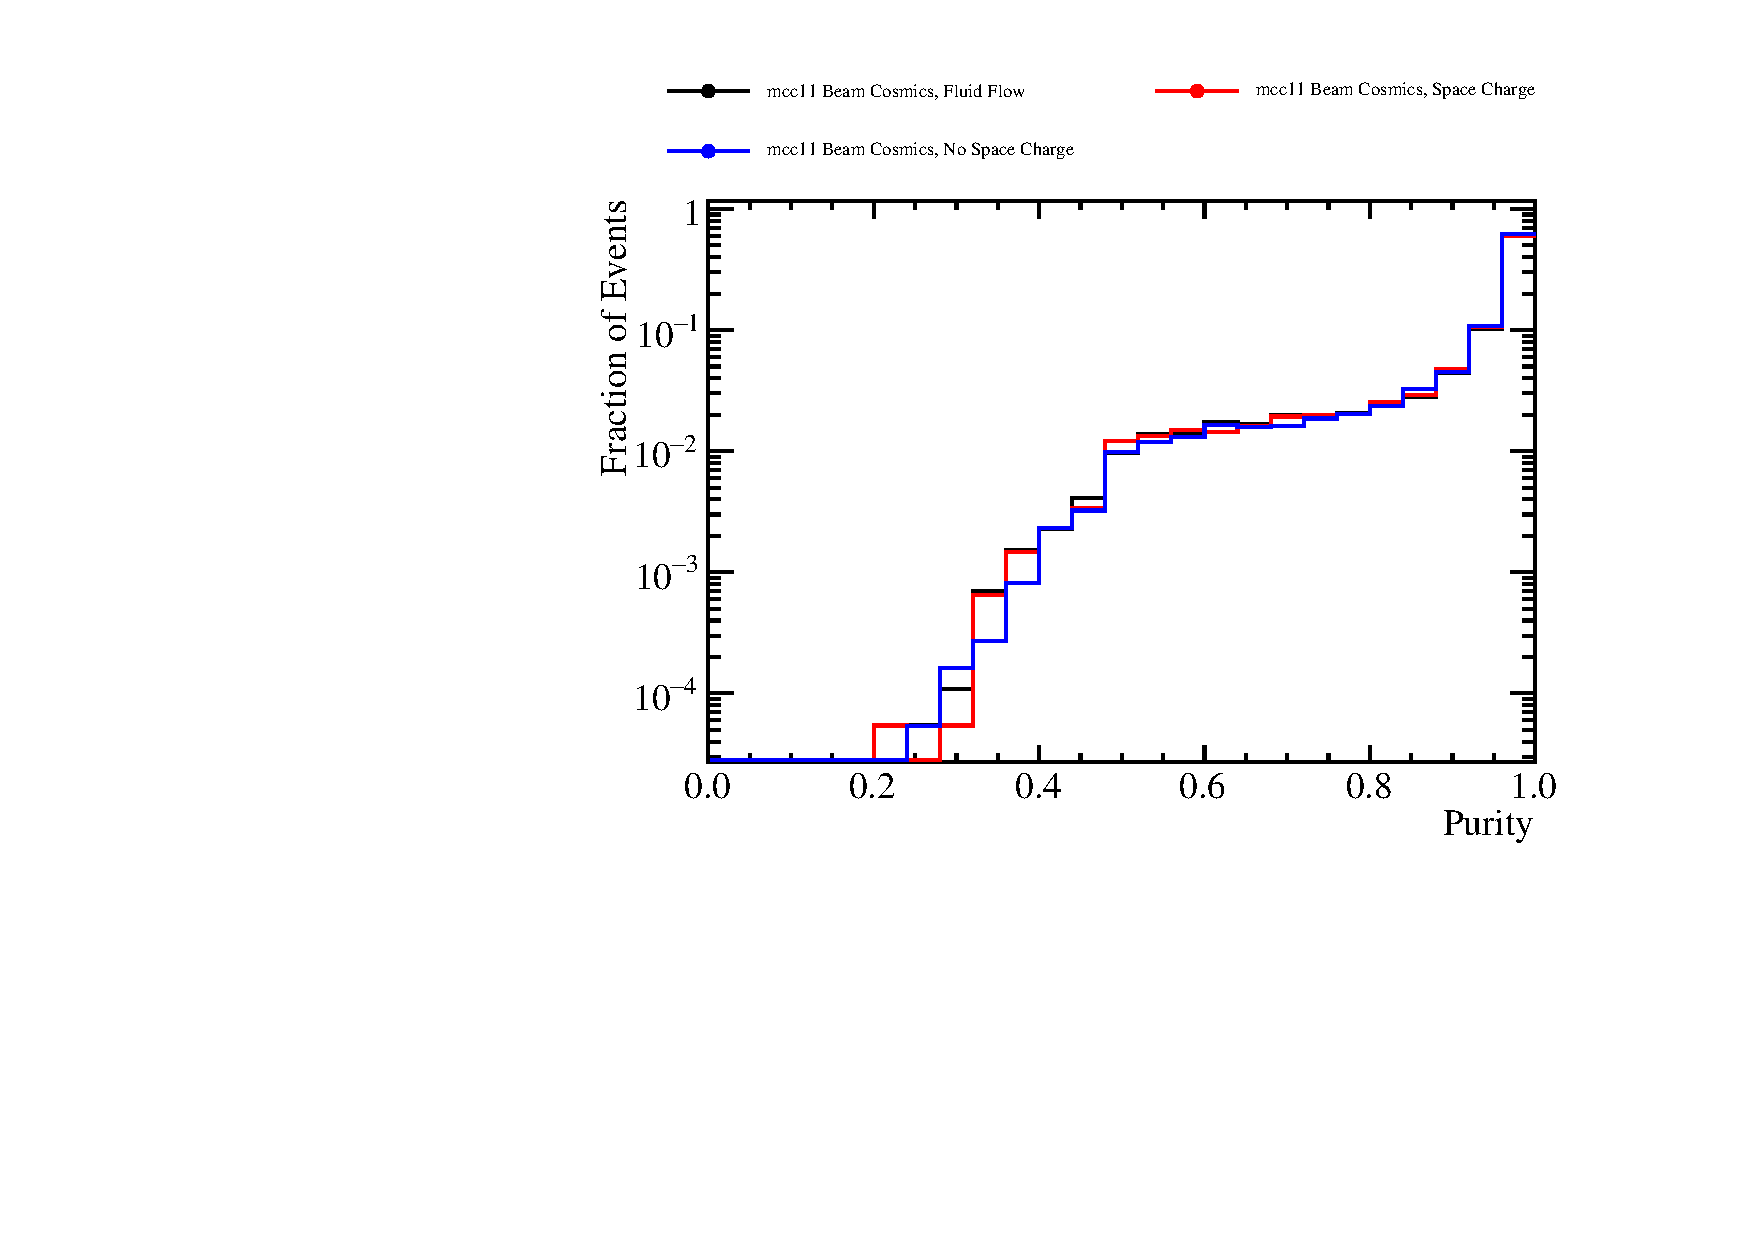
\includegraphics[width=0.5\textwidth]{Figures/Metrics/MC/Beam/BeamParticlePurity.pdf}
\caption{Please write your figure caption here}
\label{fig:2}
\end{figure}

\subsubsection{Cosmic Ray Metrics}

\begin{figure}
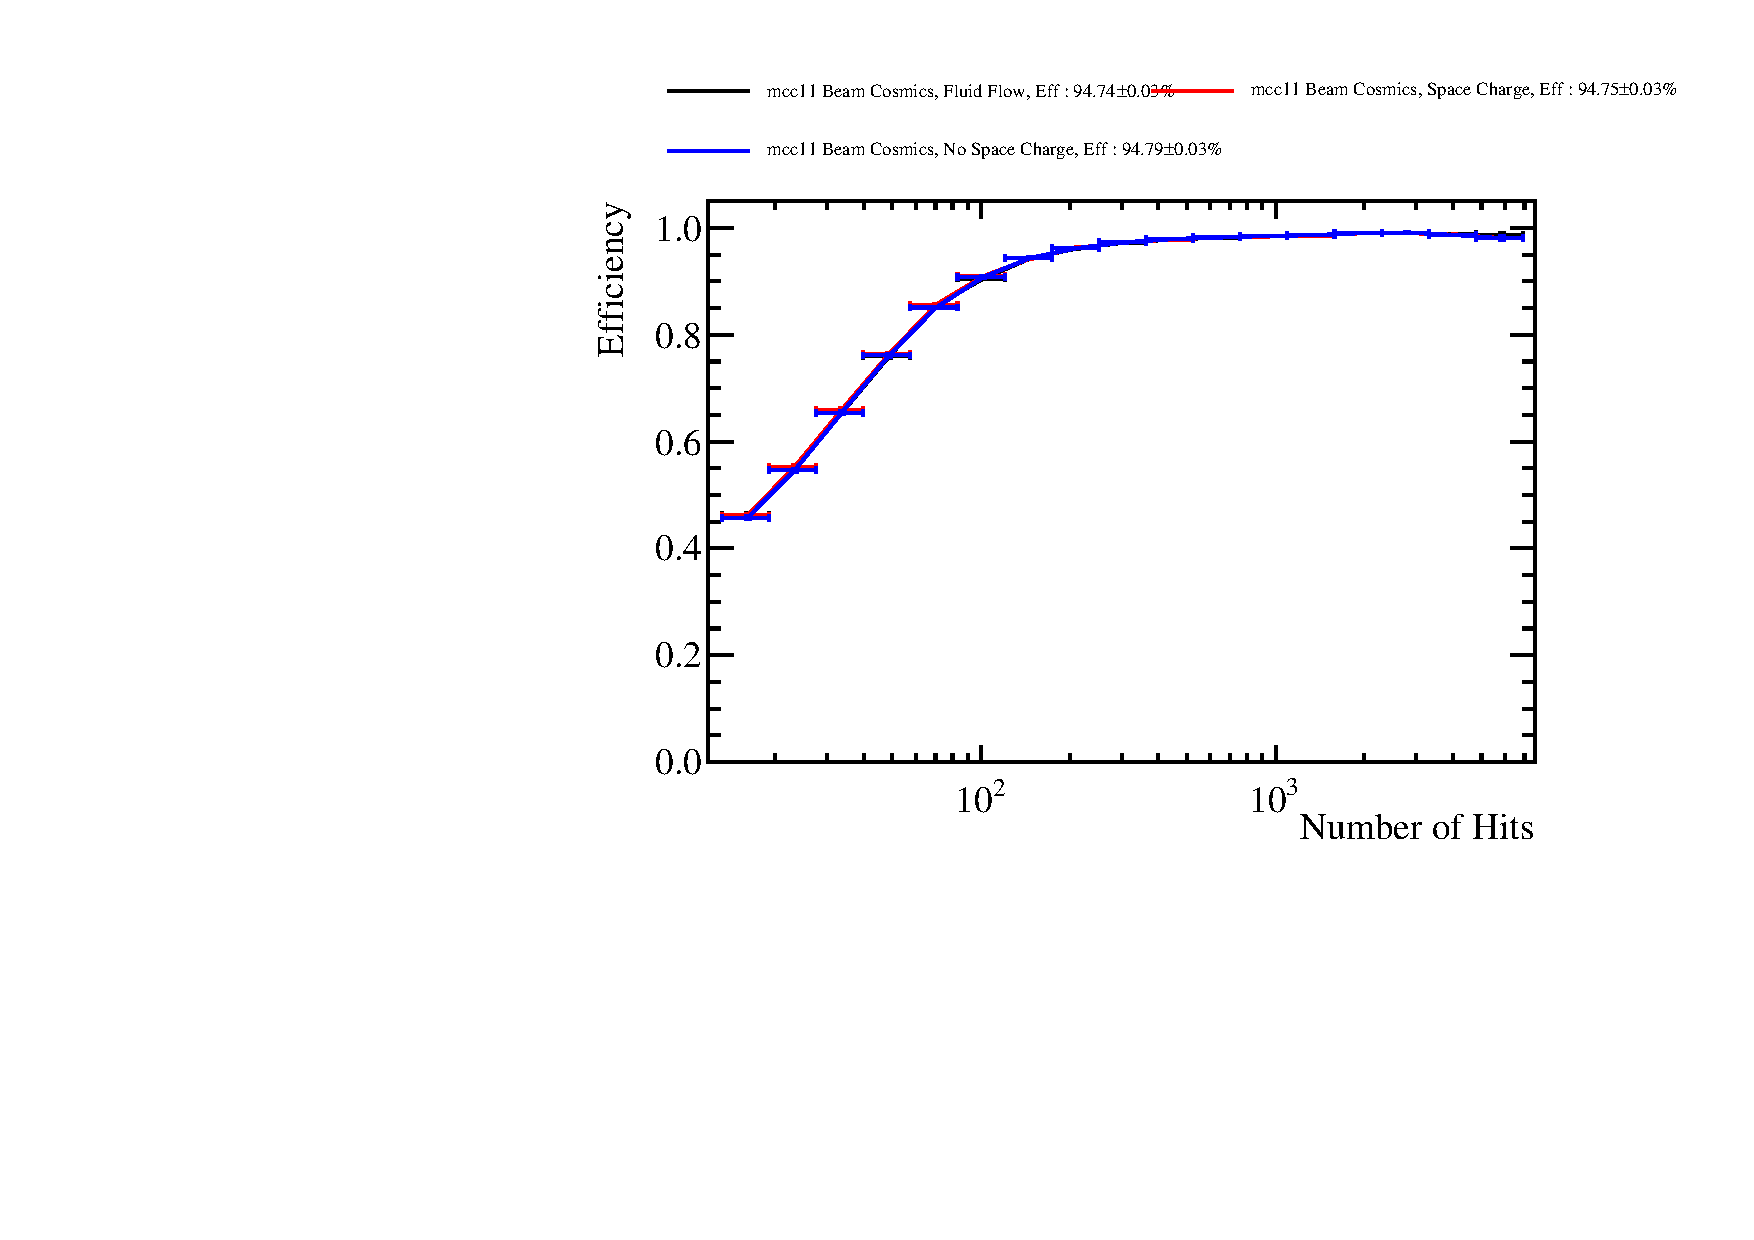
\includegraphics[width=0.75\textwidth]{Figures/Metrics/MC/Cosmics/CosmicRayEfficiencyVsNHits.pdf}
\caption{Please write your figure caption here}
\label{fig:3}
\end{figure}

\begin{figure}
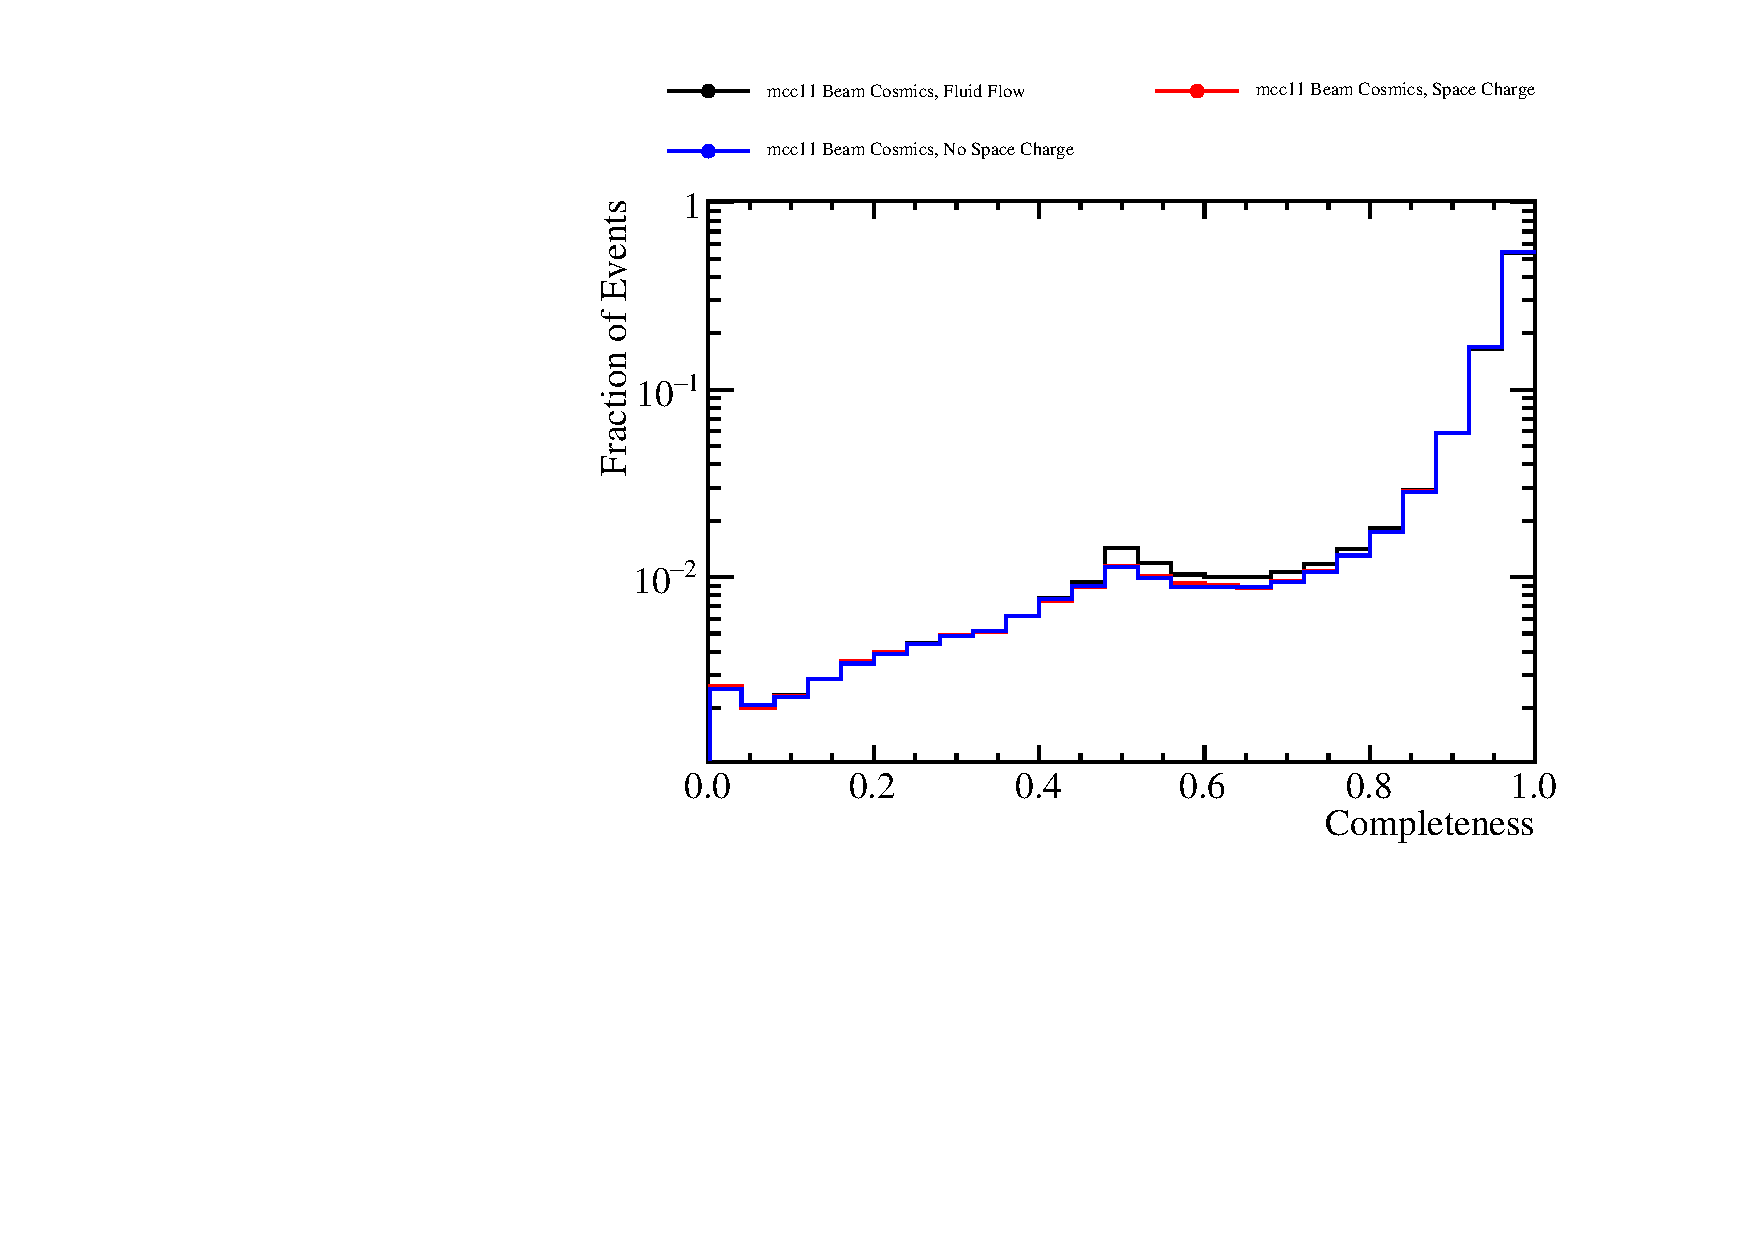
\includegraphics[width=0.5\textwidth]{Figures/Metrics/MC/Cosmics/CosmicRayCompleteness.pdf}
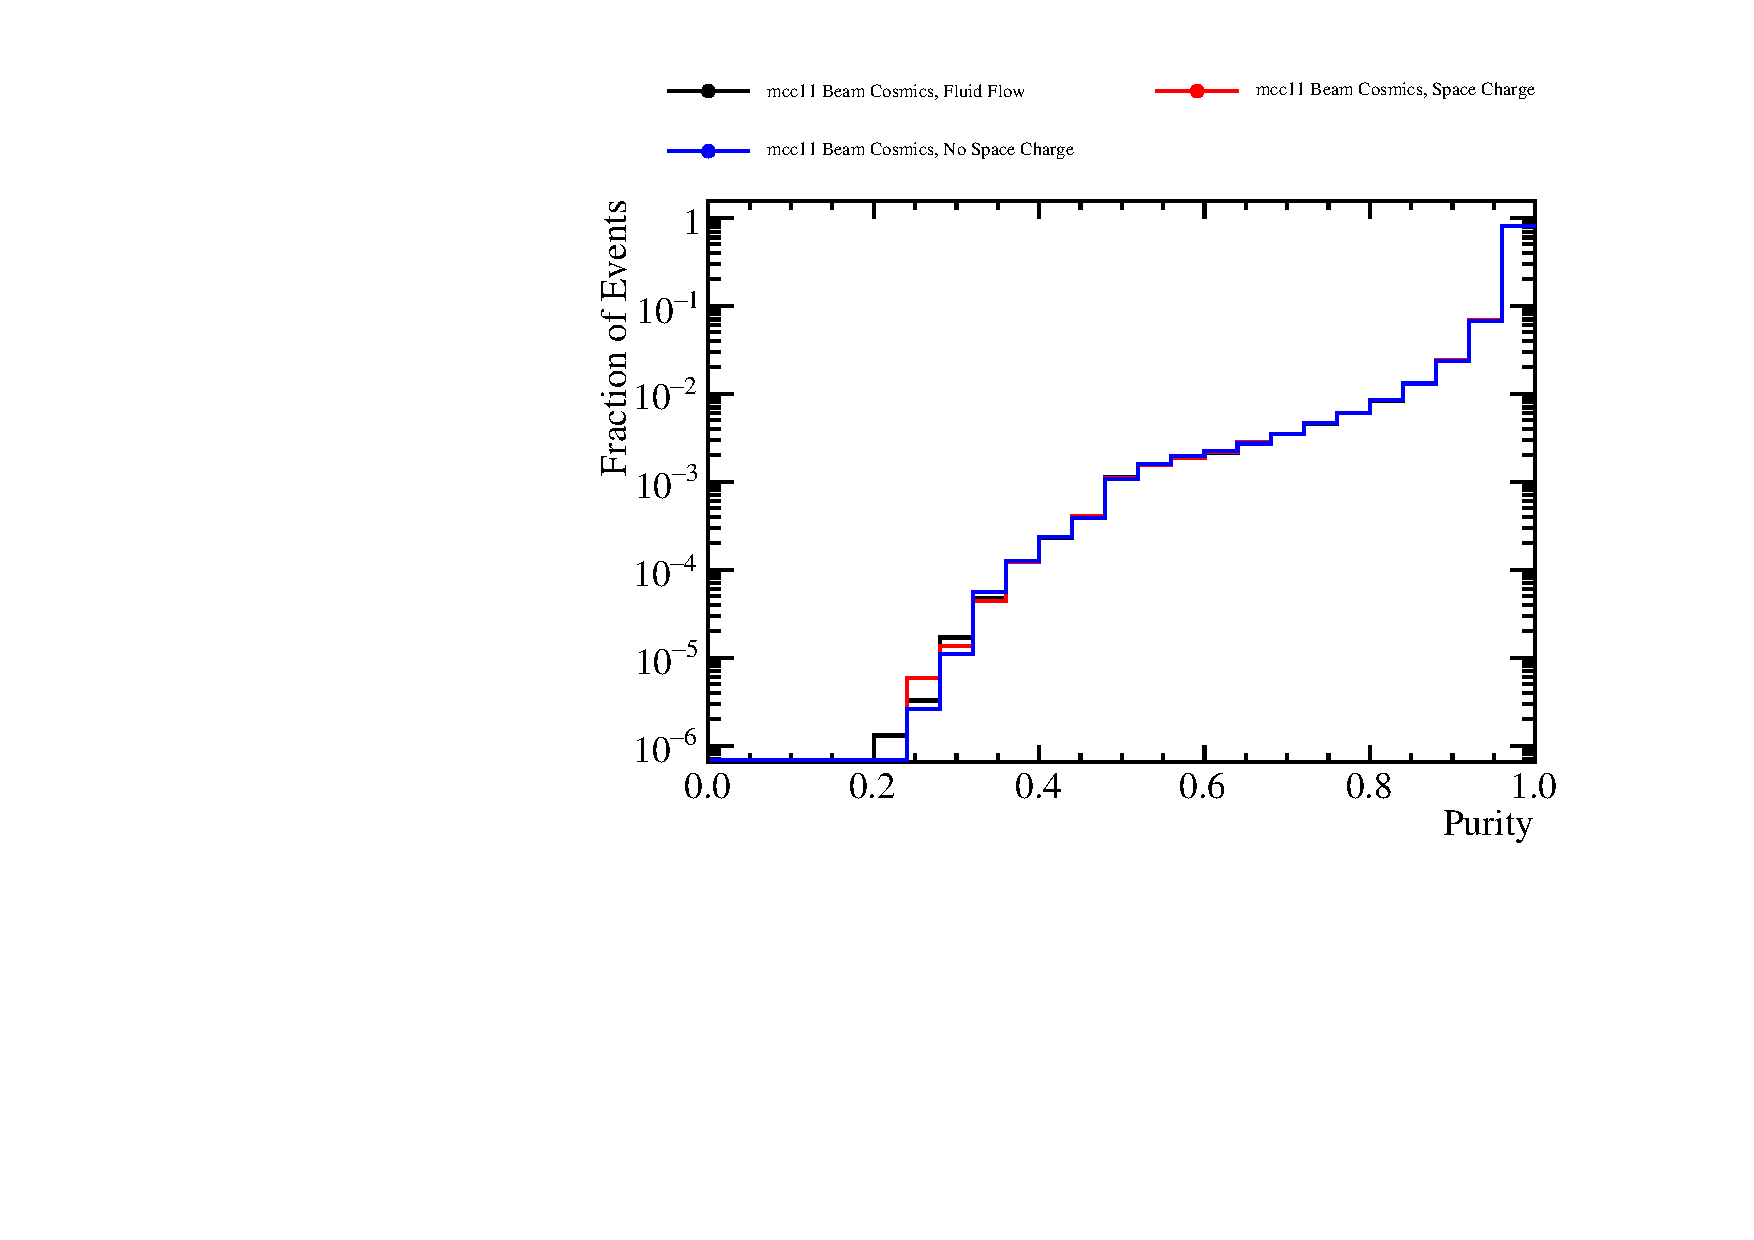
\includegraphics[width=0.5\textwidth]{Figures/Metrics/MC/Cosmics/CosmicRayPurity.pdf}
\caption{Please write your figure caption here}
\label{fig:4}
\end{figure}

\subsection{Data}

\subsubsection{Test Beam Metrics}

\begin{figure}
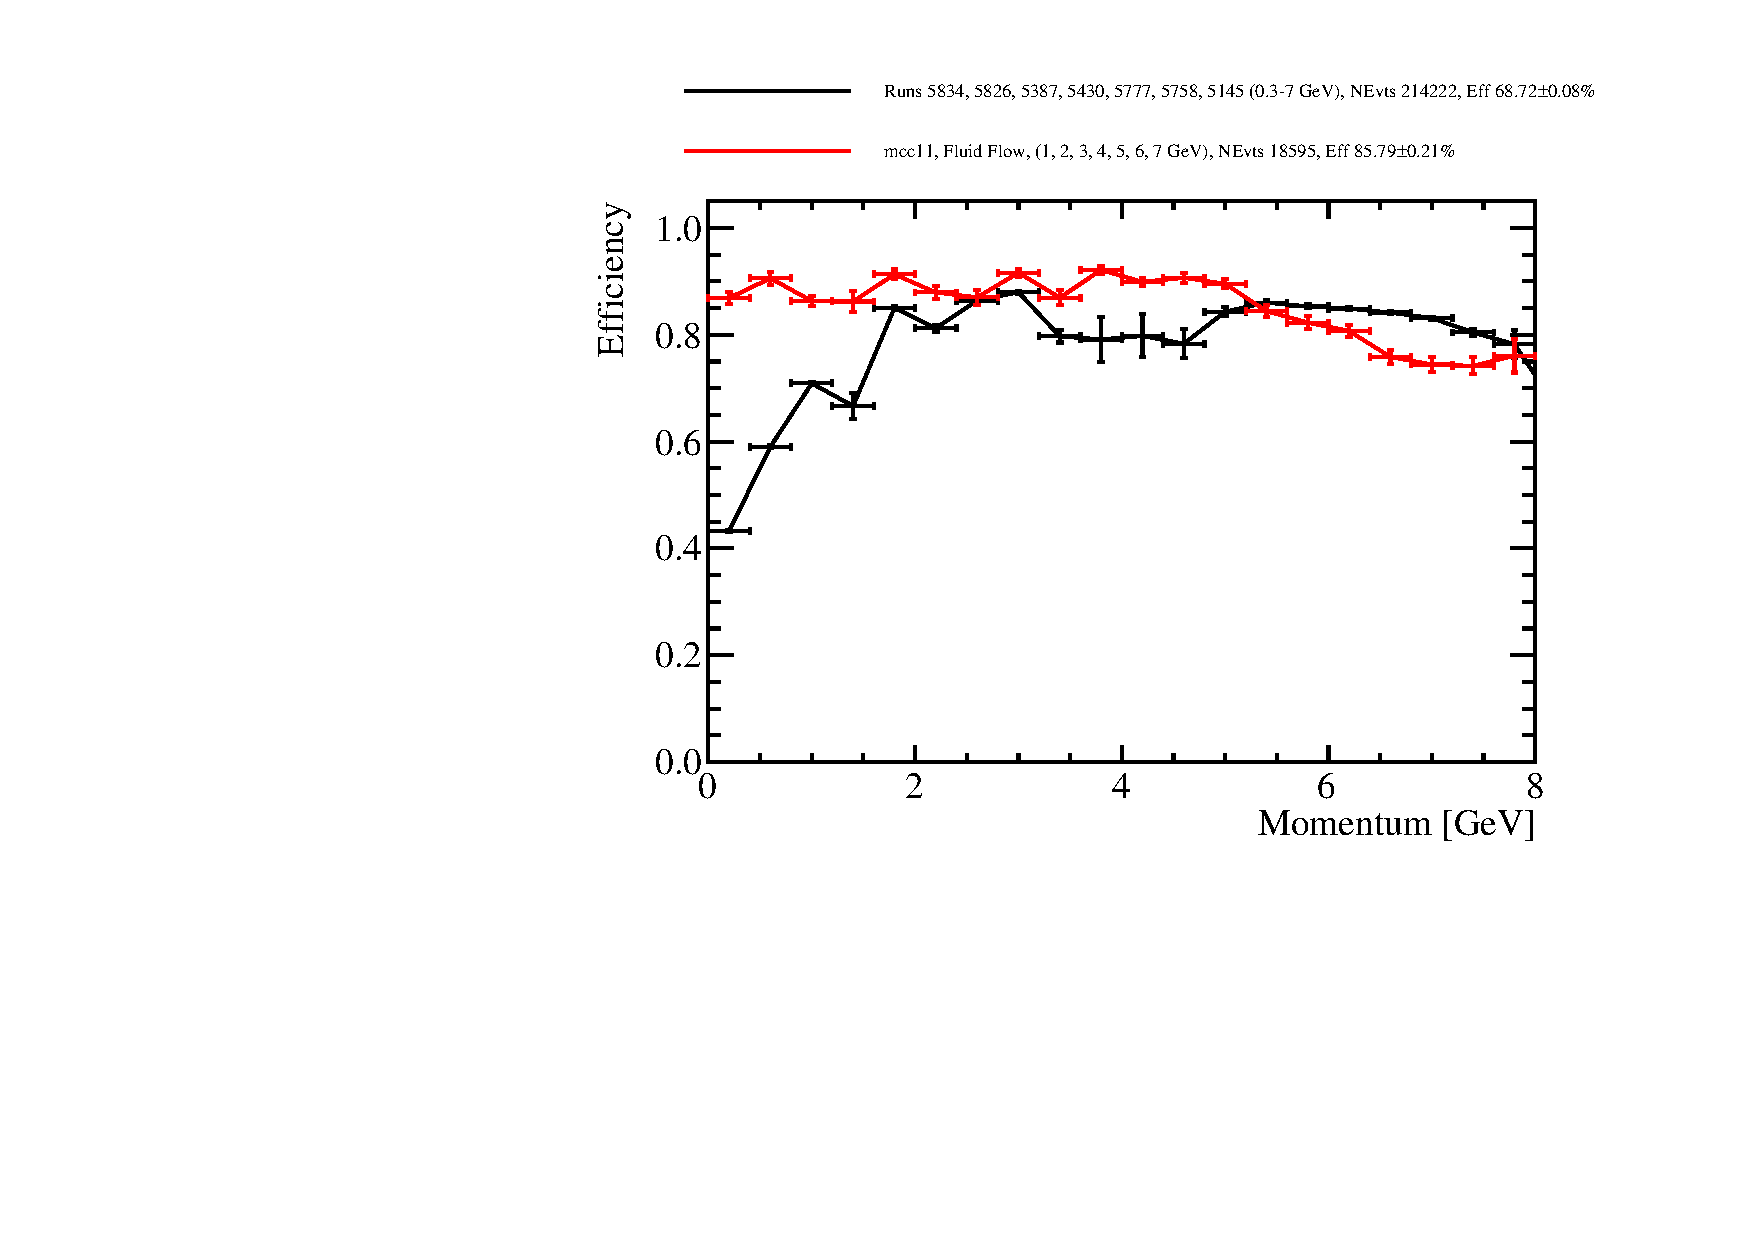
\includegraphics[width=1.0\textwidth]{Figures/Metrics/Data/Beam/BeamParticleEfficiencyVsMomentum.pdf}
\caption{Please write your figure caption here}
\label{fig:5}
\end{figure}

\begin{figure}
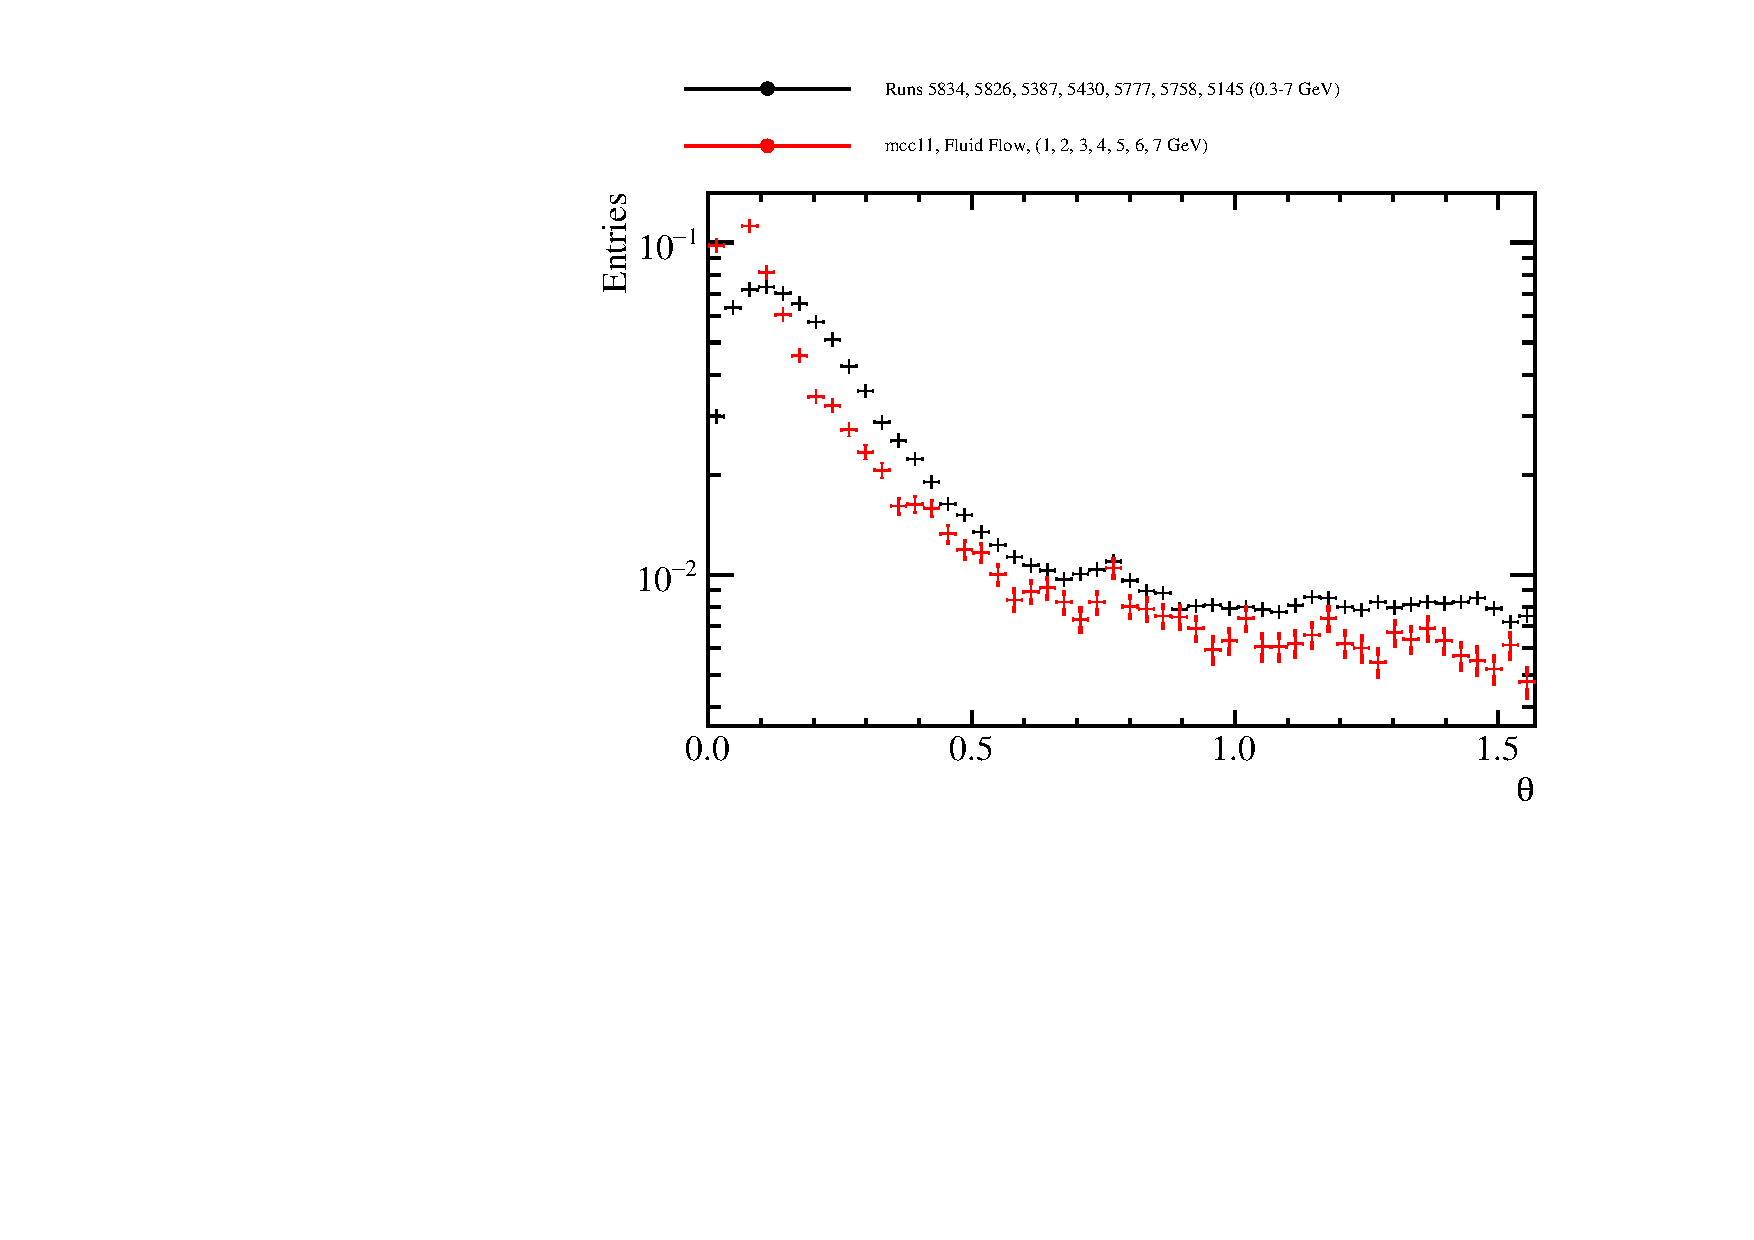
\includegraphics[width=1.0\textwidth]{Figures/Metrics/Data/Beam/BeamParticleOpeningAngle.pdf}
\caption{Please write your figure caption here}
\label{fig:6}
\end{figure}

\subsubsection{Cosmic Ray Metrics}

\begin{figure}
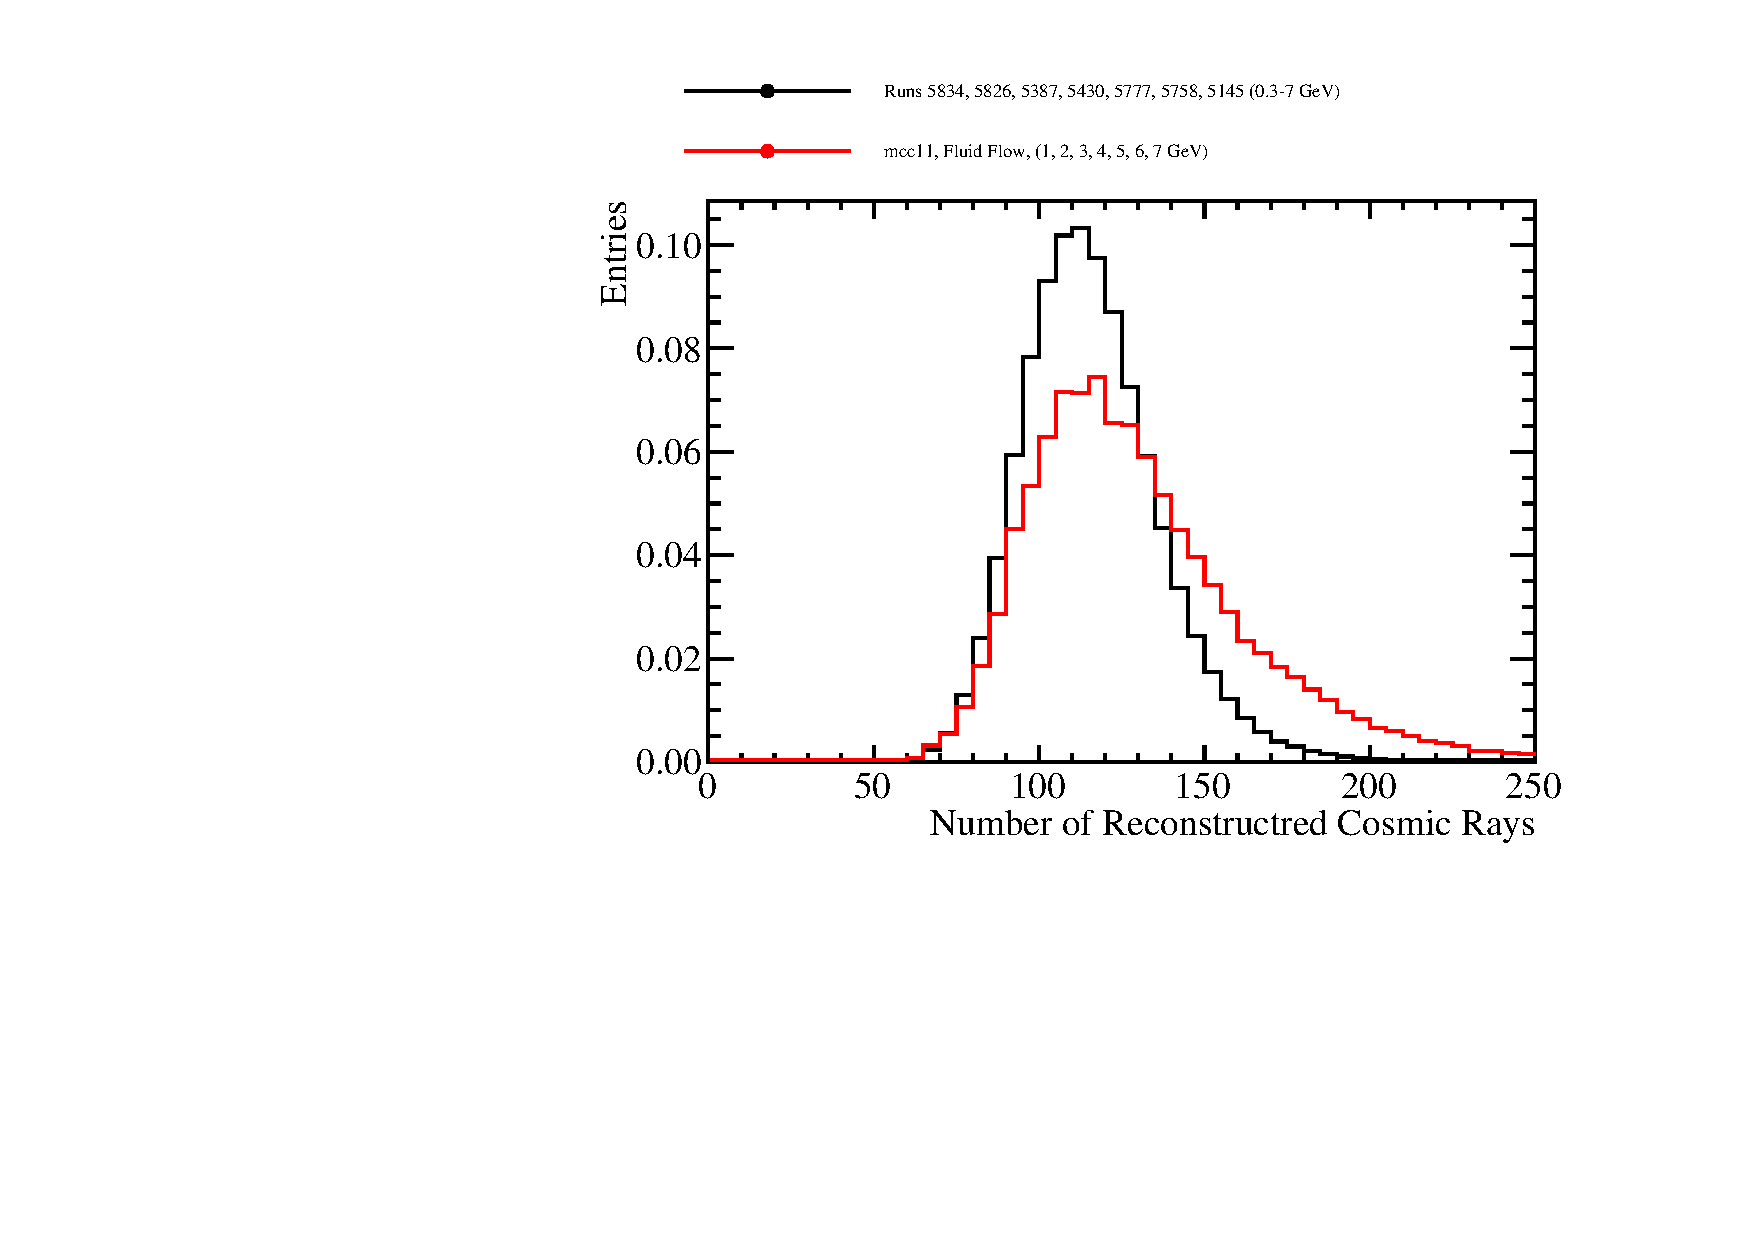
\includegraphics[width=1.0\textwidth]{Figures/Metrics/Data/Cosmics/NumberofReconstructedCosmicRays.pdf}
\caption{Please write your figure caption here}
\label{fig:7}
\end{figure}

\begin{figure}
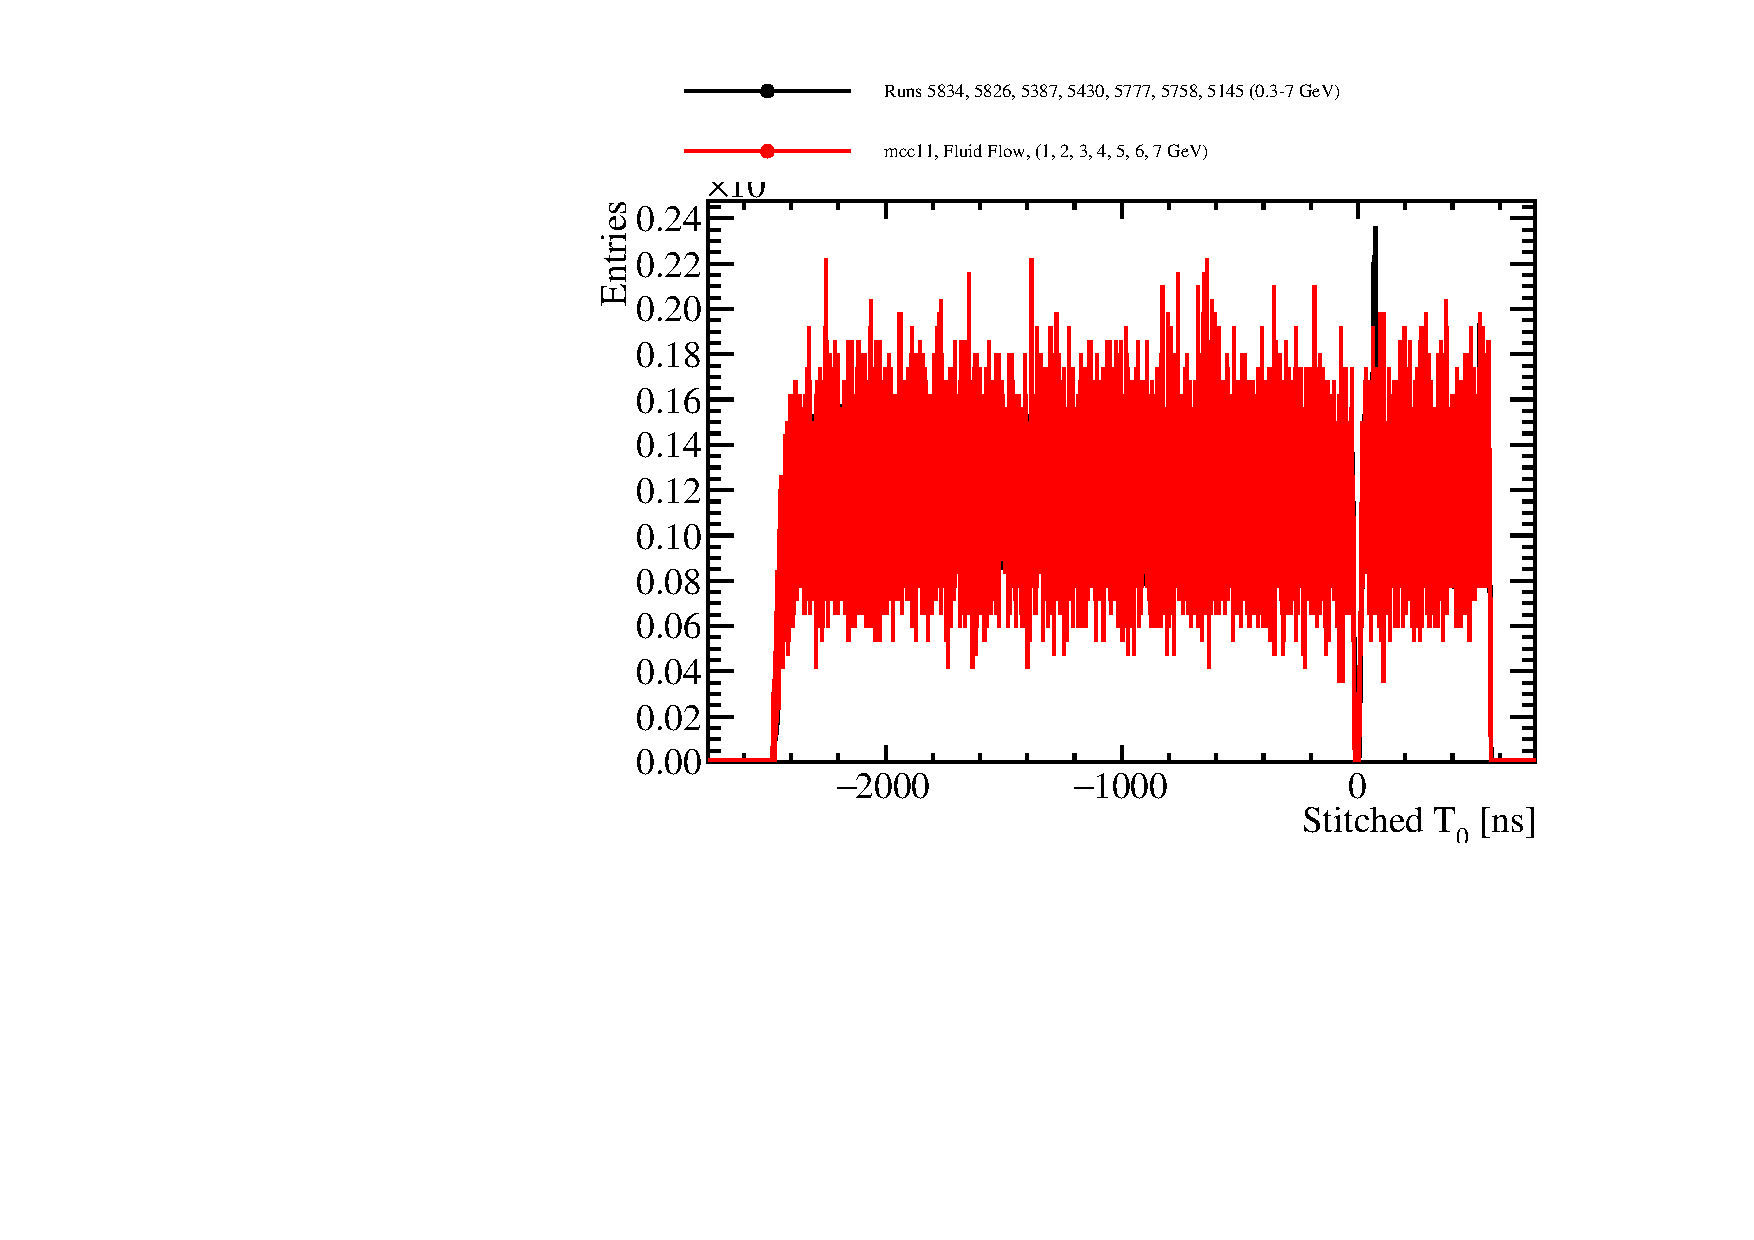
\includegraphics[width=1.0\textwidth]{Figures/Metrics/Data/Cosmics/StitchedT0.pdf}
\caption{Please write your figure caption here}
\label{fig:8}
\end{figure}

\section{Conclusions}

% For tables use
\begin{table}
% table caption is above the table
\caption{Please write your table caption here}
\label{tab:1}       % Give a unique label
% For LaTeX tables use
\begin{tabular}{lll}
\hline\noalign{\smallskip}
first & second & third  \\
\noalign{\smallskip}\hline\noalign{\smallskip}
number & number & number \\
number & number & number \\
\noalign{\smallskip}\hline
\end{tabular}
\end{table}


%\begin{acknowledgements}
%If you'd like to thank anyone, place your comments here
%and remove the percent signs.
%\end{acknowledgements}

% BibTeX users please use one of
%\bibliographystyle{spbasic}      % basic style, author-year citations
%\bibliographystyle{spmpsci}      % mathematics and physical sciences
%\bibliographystyle{spphys}       % APS-like style for physics
%\bibliography{}   % name your BibTeX data base

% Non-BibTeX users please use
\begin{thebibliography}{}
%
% and use \bibitem to create references. Consult the Instructions
% for authors for reference list style.
%
\bibitem{RefJ}
% Format for Journal Reference
Author, Article title, Journal, Volume, page numbers (year)
% Format for books
\bibitem{RefB}
Author, Book title, page numbers. Publisher, place (year)
% etc
\end{thebibliography}

\end{document}
% end of file template.tex

